% ---------------------------------------------- Preamble --------------------------------------------------------------

\documentclass{article}

% Load the packages you're going to use
\usepackage{import}                     % This package allows us to import files.
\usepackage{adjustbox}                  % This package allows you to adapt table and figure sizes to fit the page and is required by iebaltab
\usepackage{setspace}
\usepackage{hyperref}                   % Making table of contents/figures/tables clickable, so you get to exactly that section.
\usepackage{float}						% This package allows us
\usepackage{graphicx}
\usepackage{subcaption}

% Formatting packages
\doublespacing                          % Comment out (write % at the beginning of the line) to use single spacing
\usepackage{indentfirst}	            % Indents the fist paragraph of each section
\usepackage{parskip}                    % This packages sets the spacing between two paragraphs
\setlength{\parskip}{.5\baselineskip}   % Define spacing between two paragraphs

% ADD YOUR PROJECT INFO HERE
\title{Project ABC \\ Subtitle XYZ} 	%Double backslash starts a new line in \LaTeX
\author{Your Name}
\date{\today}
%\date{}                   				% Uncomment this to not print date or insert specific date

% --------------------------------------------- Preamble ends here ----------------------------------------------------

\begin{document}

\maketitle
\tableofcontents

\newpage
\listoffigures
\listoftables

\newpage
\section{Introduction} %The titles are created automatically after using this command. This command is also useful as you can create a table of content just by using this. There is no need to do anything extra.

This template was created to make your life easier. Using it, you can create a file using tables and images created in Stata. If you want to update your results, there's no need to export the tables to excel, then format them and copy into word every time. You can just run your do-file and then recompile you \LaTeX document. It will use the updated file exported by Stata and created a PDF.

You can use \LaTeX to
\begin{itemize} %Itemize creates a list of items. Like a bullet point list. You can also use enumerate which creates a list which is enumerated items which is shown as an example below.
	\item Create documentation for your project
	\item Display descriptive statistics
	\item Export regression results
	\item Share graphs
	\item Create reports that are frequently updated by just running the do-file and recompiling the report
\end{itemize}

You can also do this:
\begin{enumerate}
	\item enumerate items
	\item enumerated item number 2
\end{enumerate}

\textbf{This is a bold text.} \newline  \textit{This is an italicised text.} \\
\underline{This is an underlined text.}

%\newline starts a new line. \\ does the same.

Just pressing Enter/Return key and starting in a new line works too. Too Enter/Return keys will begin a new paragraph.

%This is a comment. I can write anything here and nobody will be able to see it except me.

\newpage
\section{Balance tests: iebaltab}
    	\input{Raw/balance_table.tex}        % This imports the table exported by Stata: add the file name

\section{Sample sizes}
	\begin{table}[H]
		\centering
		\caption{Sample sizes}
		%\begin{adjustbox}{max width=\textwidth}
			\subimport{Raw/}{samplesizes}
		%\end{adjustbox}
	\end{table}

\section{Descriptive statistics}

	\begin{table}[H]
		\centering
		\caption{Descriptive statistics for numeric variables}
		%\begin{adjustbox}{max width=\textwidth}
			\subimport{Raw/}{stats_final}
		%\end{adjustbox}
	\end{table}

	\begin{table}[H]
		\centering
		\caption{Descriptive statistics for categorical variables}
		\begin{adjustbox}{max width=\textwidth}
			\subimport{Raw/}{categorical}
		\end{adjustbox}
	\end{table}

\section{Regression tables}

	\begin{table}[H]
		\centering
		\caption{Outcome variable: life expectancy at birth}
		\begin{adjustbox}{max width=\textwidth}
			\subimport{Raw/}{regression_table}
		\end{adjustbox}
	\end{table}

 \section{Manual table}

\begin{table}[h!]                                                                       % Table starts here
	\caption{Crops by code}                                                             % Add table title
	\centering                                                                          % Center table
	\begin{tabular}{ccc}
		\hline\hline
		\textbf{Crop code} & \textbf{Portuguese name} & \textbf{English name} \\
		\hline
		1 &	Milho & Maize \\
		2 &	Arroz & Rice\\
		3 &	Mapira & Sorgum\\
		4 &	Mexoeira & Pearl millet\\
		5 &	Batata Reno & Potato \\
		\hline\hline
	\end{tabular}
\end{table}

\section{Importing figures}

	 \begin{figure}[H]
		\centering
		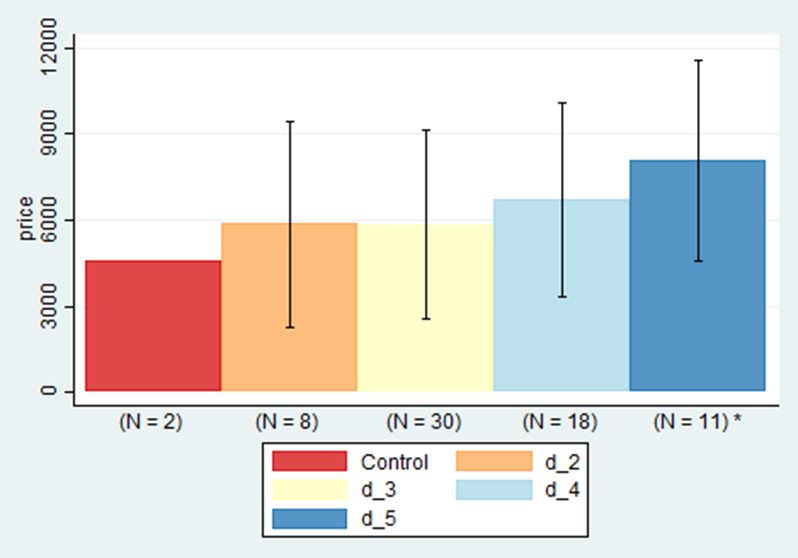
\includegraphics[width=\textwidth]{Raw/iegraph.png}
		\caption{Regular image: iegraph}  	% Add a title to the figure if you want, or leave it blank to just create a number
		\label{fig:my_label}                % Used to cross-reference figure in the document
	\end{figure}

	\begin{figure}[H]
	\centering
	\begin{subfigure}[b]{0.49\textwidth}                                  % You can adjust the size of your image here
		\includegraphics[width=\textwidth]{Raw/regular_graph.png}
		\caption{Caption below figure}                                      % Add a title to the figure or leave it blank to just create a number
	\end{subfigure}
	\begin{subfigure}[b]{0.49\textwidth}                                  % You can adjust the size of your image here
		\includegraphics[width=\textwidth]{Raw/regular_graph.png}    % This imports the image exported by stata: add the path
		\caption{Caption below figure}                                              % Add a title to the figure or leave it blank to just create a number
	\end{subfigure}
	\caption{Figure with subfigure}
\end{figure}


\end{document}
